\section{Optimointimenetelmät}

Konekoodiksi kääntäminen tuo ongelmaksi hitaan käännösvaiheen. Tämän takia modernit virtuaalikoneet sisältävät useamman kuin yhden kerroksen kääntäjiä eritasoisilla optimoinneilla. Tässä luvussa esitellään muutamia keinoja, joilla JavaScript-virtuaalikoneet ovat parantaneet kääntäjien suorituskykyä sekä niiden tuottaman konekoodin tehokkuutta.

\subsection{Piiloluokat}

\textit{Piiloluokat} (hidden classes)~\cite{v8design} ovat staattisia, eli muuttumattomia luokkia, joita virtuaalikone käyttää dynaamisten JavaScript-objektien kuvaamiseen. Jos objektia muutetaan, esimerkiksi lisäämällä siihen uusi \textit{ominaisuus} (property), luodaan sille uusi piiloluokka. Tämä kuulostaa oudolta kielen dynaamisuuden takia, mutta piiloluokkien hyödyt tulevat esiin, kun ohjelmassa on paljon samanlaisia objekteja, jotka pystyvät hyödyntämään samaa piiloluokkaa.

Kuvassa~\ref{fig:hiddenclass} näkyy esimerkki Piste-nimisen objektin ja sen piiloluokan muodostus. Kun konstruktorifunktiota kutsutaan, luodaan tyhjä objekti, jota virtuaalikone kuvaa piiloluokalla \textbf{C0}. Konstruktorissa objektiin liitetään ominaisuus x, jolloin virtuaalikone luo uuden piiloluokan \textbf{C1} ja lopulta y:n lisäyksen jälkeen \textbf{C2}:n. Seuraavalla kerralla kun luodaan uusi Piste-objekti, voidaan käyttää hyväksi olemassaolevia piiloluokkia, siirtymällä luokasta toiseen sitä mukaa kun objektia muutetaan.

\begin{figure}[ht]
    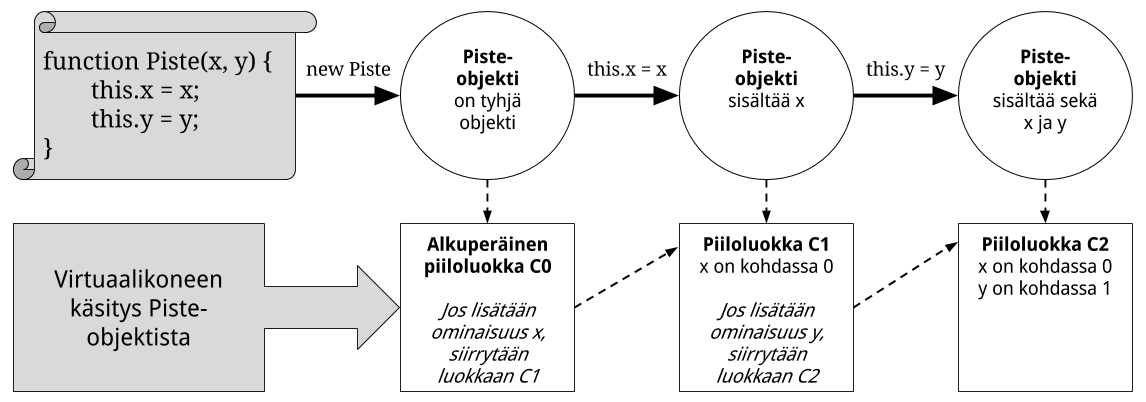
\includegraphics[width=\textwidth]{hidden-classes}
    \caption{Esimerkki piiloluokkien toimintaperiaatteesta}
     \centering
     \label{fig:hiddenclass}
\end{figure}

Piiloluokan ansiosta virtuaalikone tietää suoraan mistä muistipaikasta tieto löytyy hitaan \textit{hakurakenteen} (associative array) sijaan. Virtuaalikone voi generoida tehokkaampaa konekoodia, koska muistiviittaukset nopeutuvat huomattavasti. Jos objektia muokataan uudestaan luomisen jälkeen, täytyy optimoinnit suorittaa uudelleen. Jos kaikkia ominaisuuksia ei alusteta konstruktorissa tai niitä alustetaan ehdollisesti tuottaa myös ongelmia piiloluokkien toiminnan kannalta.

\subsection{Välimuistit}

Inline cache suomeksi?

\subsection{Roskienkeräys}

\textit{Roskienkeräys} (garbage collection) on perinteisesti toiminut melko yksinkertaisella algoritmilla nimeltään \textit{merkitse ja pyyhkäise} (mark-and-sweep)~[lähde]. Se aloittaa merkitsemisvaiheella ja lähtee liikkeelle niin sanotusta juurisetistä objekteja. Algoritmi seuraa muistiviitteitä merkiten vastaan tulleet objektit kunnes kaikki on käyty läpi. Sen jälkeen tulee pyyhkäisyvaihe. Algoritmi käy läpi koko muistin ja vapauttaa kaikki objektit mitä ei merkitty. Samalla  algoritmi poistaa merkit seuraavaa kierrosta varten.

Ohjelman suoritus ei voi jatkua roskienkeräyksen aikana ja koko muistialueen merkitseminen ja läpikäyminen on hidasta. Tämä on suuri ongelma varsinkin animaatioiden ja interaktiivisten sovellusten tapauksessa, sillä pitkä roskienkeräystauko haittaa käytettävyyttä ja saa sovelluksen tuntumaan hitaalta vaikka muu suoritus olisikin todella nopeaa.

Ongelman ratkaisemiseksi on kehitetty erilaisia heuristiikkoja ja optimointeja. Esimerkiksi \textit{sukupolveittainen roskienkeräys} (generational garbage collection) perustuu oletukseen, että suurin osa luoduista muistivarauksista ovat lyhytaikaisia. Jatkuu...

\subsection{Staattinen kertasijoitusmuoto}

%(Static single assignment form, SSA)